%%%%%%%%%%%%%%%%%%%%%%%%%%%%%%%%%%%%%%%%%%%%%%%%%%%
%% LaTeX book template                           %%
%% Author:  Amber Jain (http://amberj.devio.us/) %%
%% License: ISC license                          %%
%%%%%%%%%%%%%%%%%%%%%%%%%%%%%%%%%%%%%%%%%%%%%%%%%%%

\documentclass[a4paper,11pt]{book}

\usepackage[T1]{fontenc}
\usepackage[utf8]{inputenc}
\usepackage{lmodern}
\usepackage{hyperref}
\usepackage{graphicx}
\usepackage[portuguese]{babel}
\usepackage{amsfonts}
\usepackage[usenames,dvipsnames]{xcolor}
\usepackage{mathtools}
\usepackage{amssymb} % alguns simbolos matematicos
\usepackage{mathrsfs} % letras cursivas

% para usar definições
\usepackage{amsthm}
\theoremstyle{definition}
\newtheorem{definition}{Definição}[section]
\newtheorem{fact}{Fato}[section]
\newtheorem{demonstration}{Demonstração}[section]

% tirando identação dos paragrafos
\setlength{\parindent}{0ex}


% coding examples in latex file
\usepackage{listings}
\usepackage{xcolor}

\definecolor{codegreen}{rgb}{0,0.6,0}
\definecolor{codegray}{rgb}{0.5,0.5,0.5}
\definecolor{codepurple}{rgb}{0.58,0,0.82}
\definecolor{backcolour}{rgb}{0.95,0.95,0.92}

\lstdefinestyle{mystyle}{
    backgroundcolor=\color{backcolour},   
    commentstyle=\color{codegreen},
    keywordstyle=\color{magenta},
    numberstyle=\tiny\color{codegray},
    stringstyle=\color{codepurple},
    basicstyle=\ttfamily\footnotesize,
    breakatwhitespace=false,         
    breaklines=true,                 
    captionpos=b,                    
    keepspaces=true,                 
    numbers=left,                    
    numbersep=5pt,                  
    showspaces=false,                
    showstringspaces=false,
    showtabs=false,                  
    tabsize=2
}

\lstset{style=mystyle}

%%%%%%%%%%%%%%%%%%%%%%%%%%%%%%%%%%%%%%%%%%%%%%%%%%%%%%%%%%%%%%%%%%%%%%%%%%%%%%%%
% 'dedication' environment: To add a dedication paragraph at the start of book %
% Source: http://www.tug.org/pipermail/texhax/2010-June/015184.html            %
%%%%%%%%%%%%%%%%%%%%%%%%%%%%%%%%%%%%%%%%%%%%%%%%%%%%%%%%%%%%%%%%%%%%%%%%%%%%%%%%
\newenvironment{dedication}
{
   \cleardoublepage
   \thispagestyle{empty}
   \vspace*{\stretch{1}}
   \hfill\begin{minipage}[t]{0.66\textwidth}
   \raggedright
}
{
   \end{minipage}
   \vspace*{\stretch{3}}
   \clearpage
}

%%%%%%%%%%%%%%%%%%%%%%%%%%%%%%%%%%%%%%%%%%%%%%%%
% Chapter quote at the start of chapter        %
% Source: http://tex.stackexchange.com/a/53380 %
%%%%%%%%%%%%%%%%%%%%%%%%%%%%%%%%%%%%%%%%%%%%%%%%
\makeatletter
\renewcommand{\@chapapp}{}% Not necessary...
\newenvironment{chapquote}[2][2em]
  {\setlength{\@tempdima}{#1}%
   \def\chapquote@author{#2}%
   \parshape 1 \@tempdima \dimexpr\textwidth-2\@tempdima\relax%
   \itshape}
  {\par\normalfont\hfill--\ \chapquote@author\hspace*{\@tempdima}\par\bigskip}
\makeatother


%%%%%%%%%%%%%%%%%%%%%%%%%%%%%%%%%%%%%%%%%%%%%%%%%%%
% First page of book which contains 'stuff' like: %
%  - Book title, subtitle                         %
%  - Book author name                             %
%%%%%%%%%%%%%%%%%%%%%%%%%%%%%%%%%%%%%%%%%%%%%%%%%%%
% Book's title and subtitle
\title{\Huge \textbf{Book of Proof} \\ 
\Large Third Edition \\
\huge by Richard Hammack}

% Author
\author{\textsc{Resumo por Bruno de M. Ruas}}


\begin{document}

\frontmatter
\maketitle

\tableofcontents
%\listoffigures
%\listoftables

\mainmatter

%%%%%%%%%%%%%%%%%%%%%%%%%%%%%%%%%%%%%%%%%%%%%%%%%%%
%                    PART                         %
%%%%%%%%%%%%%%%%%%%%%%%%%%%%%%%%%%%%%%%%%%%%%%%%%%%
\part{Fundamentos}

%%%%%%%%%%%%%%%%%%%%%%%%%%%%%%%%%%%%%%%%%%%%%%%%%%%
%                 CHAPTER                         %
%%%%%%%%%%%%%%%%%%%%%%%%%%%%%%%%%%%%%%%%%%%%%%%%%%%
\chapter{Conjuntos}

\begin{chapquote}{página 3}
	``The theory of sets is a language that is perfectly suited to describing and explaning all types of mathematical structures.''
\end{chapquote}


\section*{Aviso ao Leitor}
Bem-vindo ao início de uma jornada consideravelmente longa. Esse texto é um resumo (mais conciso e menos didático) do livro do professor Hammack. O objetivo desse presente manual é servir como material de revisão e auxílio aos que quiserem seguir o caminho proposto no \textbf{Projeto Matemática} do site \href{https://economiamainstream.com.br/artigo/matematica/}{\textbf{Economia Mainstream}}. A leitura do material original é fortemente indicada e encorajada por parte dos que elaboraram o presente manual. Os exercícios contidos no livro, por outro lado, são obrigatórios. Você deve tentar resolver o máximo possível. Quaisquer dúvidas podem ser enviadas nos comentários do projeto no site citado acima.

\section{Introdução}
Um \textbf{conjunto} (set)\footnote{Eu vou intercalar bastante o uso dos termos em português e inglês.} é uma lista de \textbf{elementos}. Normalmente denotados por uma letra maiúscula. Por exemplo:

\begin{center}
	$ A = \{1 , 2 , 3 , 4 , ... \} $
\end{center}

\textbf{Regra}: Dois sets $A$ e $B$ são \textbf{iguais} se possuírem exatamente os mesmos elementos. Não importando a ordem desses elementos dentro de cada set. Ou seja, $ \{ 1,2,3 \} = \{3,1,2\}$.
\\
\\
Vamos definir um símbolo para sinalizar se um determinado elemento $(x)$ pertence ou não a um determinado set qualquer $(A)$. Para tal relação usaremos o símbolo $``\in"$ se $x$ for um elemento de $A$ ou, caso contrário, usaremos $``\notin"$ se $x$ não for um elemento de $A$.
\\
\\
É provável que, em algum momento, seja necessário contar a quantidade de elementos em um dado set qualquer $A$. Chamaremos essa relação de \textbf{cardinalidade} ou \textbf{tamanho} do set $A$. O símbolo usado será duas barras em volta do set do seguinte modo: $``|A|"$.
\\
\\
A partir dessas duas relações já podemos definir um tipo especial de set. Vamos definir como \textbf{conjunto vazio} ou \textbf{empty set} um conjunto que possua o cardinal igual a zero. Usaremos o símbolo $`` \ \emptyset \ "$ para definir a relação a seguir:

\begin{center}
	$|\emptyset| = 0$
\end{center}

Em várias situações não vale a pena construir sets apenas com uma lista-exemplo de alguns dos seus elementos. Imagine um set de todos os números pares, por exemplo, ou um set de todos os números que começam com $3$ e terminam com $4$ ou qualquer outra regra mais específica. Para essas situações usamos a \textbf{notação de formação de conjuntos (set builder notation)}. Como no exemplo abaixo:

\begin{center}
	$ E = $ \textcolor{red}{$\{$} \textcolor{blue}{$2n$} \textcolor{OliveGreen}{$:$} \textcolor{Brown}{$n$} \textcolor{Orange}{$\in$} $\mathbb{Z} \} $ \footnote{Aprender a ler a notação de formação de conjuntos é, basicamente, aprender a ler Matemática. Se esforce para entender sempre que usarmos essa técnica na hora de definir conjuntos. Para ajudar, eu vou colocar no rodapé a leitura em alguns casos.}
\end{center}

A matemática é uma linguagem que consegue dizer muita coisa com poucos símbolos. Ao longo desse curso, você será capaz de ler esses símbolos e compreender corretamente o que o autor quis dizer por meio deles. Para facilitar essa primeira leitura, eu colori cada símbolo da expressão acima com a cor correspondente da passagem a seguir. Perceba como um pequeno símbolo pode significar bastante coisa. A leitura da expressão acima é: "O conjunto $E$ é igual ao \textcolor{red}{conjunto dos elementos da forma} \textcolor{blue}{$2n$} \textcolor{OliveGreen}{tal que} \textcolor{Brown}{$n$} \textcolor{Orange}{é um elemento do conjunto} $\mathbb{Z}$".
\\
\\
Podemos resumir essa notação de formação de conjuntos como "Conjunto = {Expressão : Regra}". É bem comum vermos notações onde os dois pontos são trocados por uma barra: "Conjunto = {Expressão | Regra}". Nesse livro o autor preferiu a notação com dois pontos.
\\
\\
Existem alguns conjuntos que são famosos ao ponto de terem nomes e símbolos próprios.
\begin{itemize}
	\item[] $\emptyset = \{ \}$. Conjunto Vazio
	\item[] $\mathbb{N} = \{ 1, 2, 3, 4, ... \}$\footnote{Perceba que, para o autor do livro, $0 \notin \mathbb{N}$. Usaremos $\mathbb{N}^0$ para expressar os naturais com o elemento 0.\href{https://www.youtube.com/watch?v=j9WmXliT0lM}{ Link para um video bacana sobre o assunto.}}. Conjunto dos Naturais
	\item[] $\mathbb{Z} = \{ ..., -2, -1, 0, 1, 2, ...  \}$. Conjunto dos Inteiros
	\item[] $\mathbb{Q} = \{ x : x = m/n, \ onde \ m,n \in \mathbb{Z} \  e \  n \neq 0 \}$. Conjunto dos Racionais\footnote{Lê-se: O set dos Racionais é igual ao conjunto dos elementos $x$ tal que $x$ é formado pela divisão de $m$ por $n$, de modo que $m$ e $n$ são número inteiros e $n$ não é zero.}
	\item[] 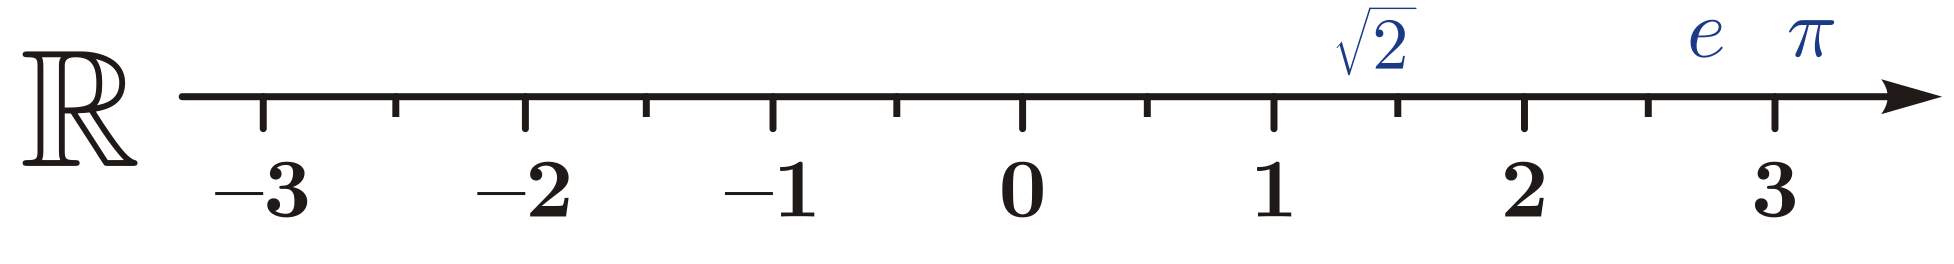
\includegraphics[scale=0.11]{images/real_line.png}. A Reta Real
\end{itemize}

Como o conjunto dos número reais pode ser descrito como pontos em uma reta numérica infinita. Se tivermos dois pontos quaisquer $a$ e $b$, de modo que $a , b \in \mathbb{R}$ e $a < b$. Temos infinitos elementos entre esses dois pontos. Por causa dessa propriedade, teremos que usar um novo símbolo para se referir aos conjuntos que são melhor descritos em termos de \textbf{intervalos} entre pontos. Abaixo coloquei uma coluna com uma representação gráfica e, ao lado, uma coluna com a respectiva definição por set builder notation.
\begin{center}
	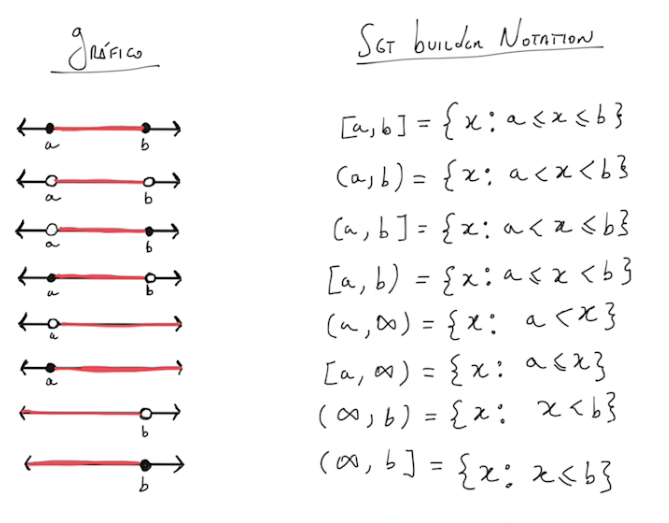
\includegraphics[scale=0.7]{images/intervals.png}
\end{center}

\section{Produto Cartesiano}
\begin{definition}[Par Ordenado]
Um \textbf{par ordenado} é um lista na forma $(x, y)$ que contém dois elementos (nesse caso, um $x$ e um $y$). Onde esses dois elementos ficam entre parênteses e separados por uma vírgula.
\end{definition}

\textbf{Regra}: Diferente dos conjuntos, a ordem dos elementos dos pares ordenados importa. Ou seja, $(x,y) \neq (y,x)$. 
\\
\\
Agora que temos a definição de par ordenado. Podemos escrever conjuntos usando esse novo conceito.

\begin{definition}[Produto Cartesiano]
O \textbf{produto cartesiano} de dois sets $A$ e $B$ é um outro set cujo símbolo é $``A \times B"$ e é definido como:
\begin{center}
$A \times B = \{ (a,b) : a \in A, b \in B \}$\footnote{Lê-se: O produto cartesiano dos conjuntos $A$ e $B$ é formado pelos pares ordenados $(a,b)$ de modo que as primeiras coordenadas são elementos de $A$ e as segundas são elementos de $B$.}
\end{center}
\end{definition}

Perceba que, se $A$ e $B$ são finitos, então $| A \times B | = |A| \ . \ |B|$. Isso é, o cardinal do produto cartesiano de dois sets é igual à multiplicação dos cardinais dos dois conjuntos.\footnote{Ao longo da etapa de Fundamentos do Projeto Matemática, faremos várias afirmações sem a devida demonstração mas, a medida que você entrar no curso de Análise, não faremos afirmações sem as devidas provas.}
\\
\\
Podemos construir um produto cartesiano onde os conjuntos $A$ e $B$ são iguais. Por exemplo: $\mathbb{R} \times \mathbb{R} = \{ (x,y) : x,y \in \mathbb{R} \}$.
\\
\\
Podemos expandir o par ordenado para infinitos elementos. Para isso vamos criar um novo conceito mais geral que abarcará o conceito de par ordenado. Chamaremos de \textbf{n-upla} a coordenada de $n$ elementos do modo $(x_1, x_2, \dots, x_n)$. Nesse conceito mais geral, um par ordenado nada mais é que uma n-upla cujo $n = 2$.
\\
\\
Para simplificar essa expressão onde temos um produto cartesiano de sets iguais, vamos criar um novo conceito que chamaremos de \textbf{potência cartesiana (Cartersian power)}. Desse modo, podemos definir o exemplo de $``\mathbb{R} \times \mathbb{R}"$ como simplesmente $``\mathbb{R}^2"$. Mais genericamente, dizemos que, para qualquer set $A$ e um $n$ positivo, o cartesian power $A^n$ será definir como:

\begin{center}
	$ A^n = \underbrace{A \times A \times ... \times A}_\text{n \ vezes} = \{ (x_1,x_2, ... , x_n) : x_1,x_2, ... , x_n \in A \} $ \footnote{Lê-se: A potência cartesiana $A^n$ é igual ao conjunto das n-uplas cujas $n$ coordenadas são elementos do conjunto $A$.}
\end{center}

\section{Subconjuntos}
Nós já aprendemos a relacionar elementos e conjuntos mas agora vamos definir um método de relacionar conjuntos entre si. A primeira relação que vamos explorar é a que expressa a situação onde todos os elementos de um conjunto também são elementos de outro conjunto.

\begin{definition}[Subconjunto]
Suponha que existam dois sets $A$ e $B$. Se todos os elementos de $A$ também forem elementos de $B$, dizemos que $A$ é um \textbf{subconjunto (subset)} de $B$. O símbolo usado para expressar essa relação é $``\subseteq"$, ou seja, $A \subseteq B$ quer dizer que $A$ é subconjunto de $B$. Caso exista um elemento de $A$ que não seja um elemento de $B$, então escrevemos que $A \nsubseteq B$.
\end{definition}

\textbf{Atenção 1}: Uma consequência direta dessa definição de subconjunto é o fato que $\emptyset \subseteq B$ para qualquer conjunto $``B"$. A demonstração dessa afirmação é simples: Suponha que exista algum conjunto $Z$ onde $\emptyset \nsubseteq Z$. Isso significaria que existe algum $x \in \emptyset$ que não é um elemento de $Z$, ou seja, $x \notin Z$. Mas, por definição, $x \notin \emptyset$, desse modo, $\emptyset \subseteq Z$.
\\
\\
\textbf{Atenção 2}: É trivial o fato que dado um conjunto qualquer $A$, todos os elementos de $A$ pertencem a ele mesmo. Isso implica que $A \subseteq A$. Portanto, todo conjunto é subconjunto de si mesmo.
\\
\\
\textbf{Atenção 3}: Como vimos antes: $\emptyset \subseteq B$, para qualquer set B. Acontece que também é verdadeiro o fato que $\emptyset \subseteq \emptyset$. Uma vez que, se $\emptyset \nsubseteq \emptyset$ existiria algum $x$ de modo que $x \in \emptyset$ e $x \notin \emptyset$. O que é uma clara contradição.

\section{Conjunto de Partes}
\begin{definition}[Conjunto de Partes]
Dado um set qualquer $B$, o seu \textbf{conjunto de partes} ou \textbf{power set} será outro set escrito como $\mathscr{P}(B)$ e definido como:
\begin{center}
	$\mathscr{P}(B) = \{ X : X \subseteq B \}$
\end{center}
\end{definition}

\textbf{Dica}: Tem bastante informação interessante no livro. Como esse aqui é só um resumo, não vou entrar muito além da definição. Mas recomendo a leitura do material original.

\section{União, Intersecção e Diferença}
Já vimos como podemos relacionar conjuntos por \textbf{produto cartesiano} para gerar outros conjuntos. Agora vamos expandir ainda mais nosso ferramental de operações entre conjuntos.

\begin{definition}[União]
Dados dois conjuntos $F$ e $G$. A \textbf{união} entre eles será um novo set denotado por $``F \cup G"$ e definido como:
\begin{center}
	$F \cup G = \{ x : x \in F \ ou \ x \in G \}$
\end{center}
\end{definition}

\begin{definition}[Intersecção]
Dados dois conjuntos $F$ e $G$. A \textbf{intersecção} entre eles será um novo set denotado por $``F \cap G"$ e definido como:
\begin{center}
	$F \cap G = \{ x : x \in F \ e \ x \in G \}$
\end{center}
\end{definition}

\begin{definition}[Diferença]
Dados dois conjuntos $F$ e $G$. A \textbf{diferença} entre eles será um novo set denotado por $``F - G"$ e definido como:
\begin{center}
	$F - G = \{ x : x \in F \ e \ x \notin G \}$
\end{center}
\end{definition}

\textbf{Dica}: Esses conceitos são muito importantes. Mas pro curso não ficar muito grande, vou me manter só nos conceitos também. Vá ler o material original caso tenha dificuldade.

\section{Complemento}
Quando lidamos com conjuntos é comum supor que há um conjunto maior que contém todos os outros. A esse set geral chamamos de \textbf{conjunto universo} ou \textbf{conjunto universal}.

\begin{definition}[Complemento]
Dado um conjunto qualquer $H$ e o seu conjunto universo $U$. O \textbf{complemento} de $H$ é um novo set denotado por $``\overline{H}"$ e definido por:
\begin{center}
	$\overline{H} = U - H$
\end{center}
\end{definition}

\section{Diagramas de Venn}

Essa sessão eu pulei integralmente. Diagramas de Venn são ótimos pra se ter uma intuição sobre todos os conceitos que vimos até agora. Mas não são usados para provas matemáticas. Ainda vale a leitura do capítulo.

\section{Conjuntos Indexados}
As vezes é necessário trabalhar com uma quantidade consideravelmente grande de conjuntos. Para esses casos, usamos uma técnica de simplificação que é adicionar um índice numérico subscrito à alguma letra maiúscula. Desse modo, ao invés de trabalharmos com sets $A$, $B$ e $C$, podemos trabalhar com os sets $A_1$, $A_2$ e $A_3$.
\\
\\
Podemos relacionar esses subscritos à um outro set. O nome dado a esse set é \textbf{conjunto índice (index set)}. Nos exemplos acima, podemos dizer que todos os subscritos pertencem ao conjunto $\{ 1 , 2 , 3 \}$.
\\
\\
Agora podemos adicionar essa técnica às relações de união e intersecção entre esses conjuntos indexados para um numero arbitrariamente grande. Além disso, vamos usar uma notação similar a do somatório\footnote{\href{https://pt.khanacademy.org/math/algebra2/sequences-and-series/alg2-sigma-notation/v/sigma-notation-sum}{Link para uma aula sobre a notação Sigma.}} para definir essas relações.

\begin{definition}[União de Sets Indexados]
Dados os conjuntos $A_1$, $A_2$, $A_3$, $\dots$, $A_n$ e o index set $I = \{ 1 , 2 , \dots , n \}$, temos que
\begin{center}
	$\bigcup_{i \in I}\limits = \{ x : x \in A_i \ para \ algum \ A_i, \ onde \  i \in I \}$
\end{center}
\end{definition}

\begin{definition}[Intersecção de Sets Indexados]
Dados os conjuntos $A_1$, $A_2$, $A_3$, $\dots$, $A_n$ e o index set $I = \{ 1 , 2 , \dots , n \}$, temos que
\begin{center}
	$\bigcap_{i \in I}\limits = \{ x : x \in A_i \ para \ todo \ A_i, \ onde \  i \in I \}$
\end{center}
\end{definition}

O livro tem dois exemplos bem interessantes da aplicação dos conceitos que acabamos de definir. A essa altura você deve conseguir entender os dois.

\section{Conjuntos que são Sistemas Numéricos}

A maioria dos conjuntos que trabalhamos são conjuntos que possuem estruturas e propriedades especiais. No caso dos conjuntos numéricos tomamos como certo que os seus elementos podem ser somados, multiplicados e possuem relações que obedecem as regras que passamos todo o ensino infantil, fundamental e médio aprendendo e aplicando. Como esse livro é introdutório, todas essas características clássicas dos sistemas numéricos serão tomadas como verdade. Mas saiba que as relações que achamos ser naturais possuem comprovações bastante complexas que você pode procurar por conta própria.
\\
\\
Aqui o autor elenca algumas propriedades que tomaremos como verdades sem que sejam devidamente definidas e demonstradas:
\begin{itemize}
	\item Propriedade Comutativa/Associativa/Distributiva da Adição/Subtração/Multiplicação/Divisão
	\item Ordenação Natural dos elementos numéricos de $\mathbb{R}$
	\item Os subconjuntos de $\mathbb{N}$ obedecem ao \href{https://pt.wikipedia.org/wiki/Princ%C3%ADpio_da_boa_ordena%C3%A7%C3%A3o}{Princípio da Boa Ordenação}.
\end{itemize}

\textbf{Comentário}: Agora a gente vai adentrar um pouco nas propriedades que podemos derivar desses pressupostos acima. Pode parecer que é um papo chato, mas a sua missão é se certificar que você é capaz de compreender toda a explicação. Vença a preguiça.
\\
\\
Uma conclusão que podemos tirar do princípio da boa ordenação é que dado um conjunto não nulo qualquer $A \subseteq \mathbb{N}$ sempre vai haver um $x_0 \in A$ que seja o seu \textbf{menor elemento}. De modo parecido, para qualquer $b \in \mathbb{Z}$, qualquer conjunto não nulo $A \subseteq \{ b, b+1, b+2, b+3, \dots \}$ também possui um \textbf{menor elemento}.

\begin{fact}[Division Algorithm]
Dados dois inteiros $a$ e $b$, onde $b > 0$. Existem outros dois inteiros únicos $q$ e $r$ para qual $a = qb + r$ e $0 \leq r < b$.
\end{fact}

Agora o autor demonstra a existência de $r$ e $q$ com suas propriedades. Talvez depois eu estenda a prova para a unicidade desses valores\footnote{Passa lá no Economia Mainstream e me dá uma cobrada nos comentários}.

\begin{demonstration}[Division Algorithm - Existência de $r$ e $q$]
Dados $a,b \in \mathbb{Z}$ e $b > 0$, é possível criar um set do tipo:
\begin{center}
	$ A = \{ a - xb : x \in \mathbb{Z}, 0 \leq a - xb \} \subseteq \mathbb{N}^0 $
\end{center}
Desse modo, $A \subseteq \mathbb{N}^0$. Por causa disso, podemos aplicar o princípio da boa ordenação em $A$ e dizer que existe algum elemento $r$ que seja o menor elemento de $A$.
\\
\\
Como $r \in A$ ele pode ser escrito da forma $r = a - qb$ onde $x = q \in \mathbb{Z}$. Desse fato podemos tirar duas informações úteis: 1) $a = r + qb$ e 2) Como $r \in \mathbb{N}^0$, então $r \geq 0$.
\\
\\
Agora só nos resta provar que $r < b$ mas para isso, vamos usar o pensamento contrário: O que aconteceria se $r \geq b$?
\\
\\
Ora, se $r \geq b$, então a subtração $r - b$ será um número positivo, portanto será também um elemento de $\mathbb{N}^0$. Podemos reescrever essa subtração como $r - b = (a - qb) - b = a - (q + 1)b$. 
\\
\\
Mas veja só que estranho, $q + 1$ certamente será um elemento de $\mathbb{Z}$. Logo, o número expresso por $a - (q + 1)b$ também será um elemento de $A$ (nesse caso, $(q + 1)$ é o $x$). Portanto, não é possível que $r$ seja o seu menor elemento visto que $r - b$ também é um elemento de $A$ e é menor que $r$. Isso é uma clara contradição. Isso é justamente isso que queríamos mostrar: Quando tomamos $r \geq b$ acabamos com uma contradição\footnote{O nome dessa técnica é: prova por contradição. Falaremos dela mais pra frente no curso.}, portanto, só podemos aceitar o oposto, ou seja, sabemos que $r < b$. Com isso finalizamos a demonstração da existência de $r$ e $q$ com as propriedades anteriormente citadas $\blacksquare$\footnote{Esse quadrado preto é usado para pontuar o final de uma demonstração.}
\end{demonstration}

\section{O Paradoxo de Russell}

Até agora trabalhos a distinção entre "elementos" e "conjuntos". Mas, na verdade, qualquer número (ou seja, elemento de sets numéricos) pode, sim, ser interpretado como um conjunto.\footnote{Existe um mundo de teoria sobre conjuntos, nós não temos tempo pra entrar muito fundo nessa questão. Então vá atrás de livros sobre teoria dos conjuntos e seja feliz.}. Até mesmos as operações matemáticas podem ser definidas usando-se teoria dos conjuntos. O Autor vai até mais longe "Qualquer entidade matemática é um conjunto, mesmo que não escolhamos pensar desse modo".
\\
\\
Essa parte do paradoxo de Russell não serve pro resto do livro mas é bem legal de saber. O que Bertrand Russell propôs foi o seguinte conjunto:
\begin{center}
	$ A = \{ X : X $ é um set e $X \notin X \}$\footnote{Ou seja, A é formado por todos os conjuntos que não possuem a si mesmo como elemento.}
\end{center}
E perguntou: "O conjunto $A$ é um elemento de si mesmo?".
\\
\\
Acredite, apenas esse enunciado foi uma baita dor de cabeça para os matemáticos na época. Esse assunto não é necessário para a compreensão do resto desse material. Se você quiser entender um pouco mais, confira esse \href{https://www.youtube.com/watch?v=AQTTYAM8BF0}{link} ou esse outro \href{https://www.youtube.com/watch?v=0Bs0lJRxOaI}{link}.
\\
\\
\textbf{Dica}: Vai ler o livro nessa parte. O professor explica bem melhor sobre o paradoxo.

%%%%%%%%%%%%%%%%%%%%%%%%%%%%%%%%%%%%%%%%%%%%%%%%%%%
%                 CHAPTER                         %
%%%%%%%%%%%%%%%%%%%%%%%%%%%%%%%%%%%%%%%%%%%%%%%%%%%
\chapter{Lógica}

\begin{chapquote}{página 34}
	``Logic is a systematic way of thinking that allow us to parse the meanings of sentences and to deduce new information from old information. [...] Logic is  a process of deducing information correctly, not just deducing correct information''
\end{chapquote}

\section{Proposições}

O estudo da lógica começa com as proposições. Uma \textbf{proposição} é uma sentença ou expressão matemática que seja definitivamente verdadeira ou falsa. Em cima dessas proposições é que aplicamos a lógica para produção de novas proposições. Qualquer resultado ou teorema provado é, na verdade, uma proposição\footnote{Isso inclui o teorema de Pitágoras, por exemplo.}.
\\
\\
Podemos usar letras para nomear proposições. Por exemplo, a proposição "Se um número $x$ é múltiplo de 6, então $x$ é par" \  pode ser resumida em uma letra. Nesse caso diremos que "$P$" \ é a proposição acima. Dessa feita, sempre que dissermos $P$ é falso ou $P$ é verdadeiro, estamos nos referindo a proposição completa.
\\
\\
Quando uma proposição possuir variáveis, podemos escreve-la de uma maneira similar às funções. No exemplo do parágrafo acima, podemos usar o símbolo $P(x)$ para expressar que a proposição $P$ possui uma variável $x$ dentro dela.\footnote{Fique atento para não confundir quando estivermos nos referindo a funções e proposições.}
\\
\\
Uma \textbf{sentença aberta} é uma proposição cuja validade depende da sua variável. Ou seja, dependendo do valor que você der para a variável, a proposição pode ser verdadeira ou falsa.
\\
\\
O livro do professor Hammack é justamente sobre o método de como se provar que uma proposição é verdade ou falsa. Para provar uma proposição você deve começar com proposições que sejam claramente verdadeiras e usar a lógica para deduzir outras proposições mais complexas que as anteriores até que, por fim, se chegue na proposição que se quer provar.

\section{Operadores: e, ou, não}

Até agora dizemos que você pode usar proposições junto à lógica para se chegar a outras proposições. Então vamos aprender como trabalhar com mais de uma proposição por meio dos \textbf{operadores lógicos}.
\\
\\
O primeiro operador que vamos aprender é o "$e$". Dadas as proposições $P$ e $Q$. Podemos criar uma nova proposição através desse operador. Quando escrevemos $R: P \ e \ Q$, estamos criando uma nova proposição $R$ que é composta de das duas proposições $P$ e $Q$. O símbolo usado para esse conectivo é o "$\land$". Aqui em baixo vamos colocar a tabela verdade\footnote{"V" significa Verdadeiro e "F" significa Falso.} desse operador\footnote{Se você não sabe o que são tabelas-verdades então dá uma lida nesse \href{https://www.youtube.com/watch?v=hWEZsyF3ZZc}{link}.}

\begin{center}
\begin{tabular}{ c c || c }
 P & Q & $P \land Q$ \\ 
 \hline
 V & V & V \\  
 V & F & F \\  
 F & V & F \\  
 F & F & F
\end{tabular}
\end{center}

Outro operador lógico clássico é o "ou". O símbolo dele é o "$\lor$". Eu sei, parece muito com o símbolo do "e" \ mas a  gente não pode fazer nada a não ser decorar bem a distinção entre esses dois símbolos. A tabela-verdade do "ou" \ segue abaixo.

\begin{center}
\begin{tabular}{ c c || c }
 P & Q & $P \lor Q$ \\ 
 \hline
 V & V & V \\  
 V & F & V \\  
 F & V & V \\  
 F & F & F
\end{tabular}
\end{center}

\textbf{Atenção}: O significado da palavra "ou" \ na linguagem do dia a dia é diferente do significado empregado no contexto da lógica. Quando usamos o conectivo "ou" \ na lógica, fica implícita a possibilidade de ambas as proposições serem verdadeiras ao mesmo tempo. Para as situações onde queremos que apenas uma proposição seja aceita mas não ambas, usamos um "ou exclusivo"\footnote{O símbolo desse é o "$\oplus$".} \ dos seguintes modos: 

\begin{itemize}
\item ou $P$ ou $Q$
\item $P$ ou $Q$, mas não ambos
\item Exatamente um de $P$ ou $Q$
\end{itemize}

O último operador que veremos é a \textbf{negação}. Ela inverte a condição da proposição onde é aplicada. Seu símbolo é o " \~{} "\footnote{Existem outras representações desse operador: $\lnot$ , $\veebar$ , $\dot\lor$}, ou seja, se uma proposição é verdadeira, ao aplicarmos a negação à ela, tornamos essa proposição falsa. A tabela-verdade desse operador é bem simples.

\begin{center}
\begin{tabular}{ c || c }
 P & \~{}$P$ \\ 
 \hline
 V & F \\  
 F & V
\end{tabular}
\end{center}

\section{Proposições Condicionais}
\section{Proposições Bicondicionais}
\section{Tabelas-Verdade para Proposições}
\section{Equivalência Lógica}
\section{Quantificadores}
\section{Um pouco mais de Proposições Condicionais}
\section{Traduzindo Português para Lógica Simbólica}
\section{Negando Proposições}
\section{Inferência Lógica}
\section{Nota Importante}

%%%%%%%%%%%%%%%%%%%%%%%%%%%%%%%%%%%%%%%%%%%%%%%%%%%
%                 CHAPTER                         %
%%%%%%%%%%%%%%%%%%%%%%%%%%%%%%%%%%%%%%%%%%%%%%%%%%%
\chapter{Contagem}




%%%%%%%%%%%%%%%%%%%%%%%%%%%%%%%%%%%%%%%%%%%%%%%%%%%
%                    PART                         %
%%%%%%%%%%%%%%%%%%%%%%%%%%%%%%%%%%%%%%%%%%%%%%%%%%%
\part{Como Provar Afirmações Condicionais}

%%%%%%%%%%%%%%%%%%%%%%%%%%%%%%%%%%%%%%%%%%%%%%%%%%%
%                 CHAPTER                         %
%%%%%%%%%%%%%%%%%%%%%%%%%%%%%%%%%%%%%%%%%%%%%%%%%%%
\chapter{Prova Direta}

%%%%%%%%%%%%%%%%%%%%%%%%%%%%%%%%%%%%%%%%%%%%%%%%%%%
%                 CHAPTER                         %
%%%%%%%%%%%%%%%%%%%%%%%%%%%%%%%%%%%%%%%%%%%%%%%%%%%
\chapter{Prova Contra-positiva}

%%%%%%%%%%%%%%%%%%%%%%%%%%%%%%%%%%%%%%%%%%%%%%%%%%%
%                 CHAPTER                         %
%%%%%%%%%%%%%%%%%%%%%%%%%%%%%%%%%%%%%%%%%%%%%%%%%%%
\chapter{Prova por Contradição}


%%%%%%%%%%%%%%%%%%%%%%%%%%%%%%%%%%%%%%%%%%%%%%%%%%%
%                    PART                         %
%%%%%%%%%%%%%%%%%%%%%%%%%%%%%%%%%%%%%%%%%%%%%%%%%%%
\part{Mais Sobre Provas}

%%%%%%%%%%%%%%%%%%%%%%%%%%%%%%%%%%%%%%%%%%%%%%%%%%%
%                 CHAPTER                         %
%%%%%%%%%%%%%%%%%%%%%%%%%%%%%%%%%%%%%%%%%%%%%%%%%%%
\chapter{Prova de Afirmações Não-Condicionais}

%%%%%%%%%%%%%%%%%%%%%%%%%%%%%%%%%%%%%%%%%%%%%%%%%%%
%                 CHAPTER                         %
%%%%%%%%%%%%%%%%%%%%%%%%%%%%%%%%%%%%%%%%%%%%%%%%%%%
\chapter{Provas Envolvendo Conjuntos}

%%%%%%%%%%%%%%%%%%%%%%%%%%%%%%%%%%%%%%%%%%%%%%%%%%%
%                 CHAPTER                         %
%%%%%%%%%%%%%%%%%%%%%%%%%%%%%%%%%%%%%%%%%%%%%%%%%%%
\chapter{Contraprova}

%%%%%%%%%%%%%%%%%%%%%%%%%%%%%%%%%%%%%%%%%%%%%%%%%%%
%                 CHAPTER                         %
%%%%%%%%%%%%%%%%%%%%%%%%%%%%%%%%%%%%%%%%%%%%%%%%%%%
\chapter{Indução Matemática}


%%%%%%%%%%%%%%%%%%%%%%%%%%%%%%%%%%%%%%%%%%%%%%%%%%%
%                    PART                         %
%%%%%%%%%%%%%%%%%%%%%%%%%%%%%%%%%%%%%%%%%%%%%%%%%%%
\part{Relações, Funções e Cardinalidade}

%%%%%%%%%%%%%%%%%%%%%%%%%%%%%%%%%%%%%%%%%%%%%%%%%%%
%                 CHAPTER                         %
%%%%%%%%%%%%%%%%%%%%%%%%%%%%%%%%%%%%%%%%%%%%%%%%%%%
\chapter{Relações}

%%%%%%%%%%%%%%%%%%%%%%%%%%%%%%%%%%%%%%%%%%%%%%%%%%%
%                 CHAPTER                         %
%%%%%%%%%%%%%%%%%%%%%%%%%%%%%%%%%%%%%%%%%%%%%%%%%%%
\chapter{Funções}

%%%%%%%%%%%%%%%%%%%%%%%%%%%%%%%%%%%%%%%%%%%%%%%%%%%
%                 CHAPTER                         %
%%%%%%%%%%%%%%%%%%%%%%%%%%%%%%%%%%%%%%%%%%%%%%%%%%%
\chapter{Provas com Calculus}

%%%%%%%%%%%%%%%%%%%%%%%%%%%%%%%%%%%%%%%%%%%%%%%%%%%
%                 CHAPTER                         %
%%%%%%%%%%%%%%%%%%%%%%%%%%%%%%%%%%%%%%%%%%%%%%%%%%%
\chapter{Cardinalidade de Conjuntos}

\end{document}
